\documentclass{standalone}
\usepackage{pgfplots}
\usepackage{siunitx}
\usepgfplotslibrary{dateplot}
%\usepgfplotslibrary{external}
%\tikzexternalize % Enable externalization

\begin{document}

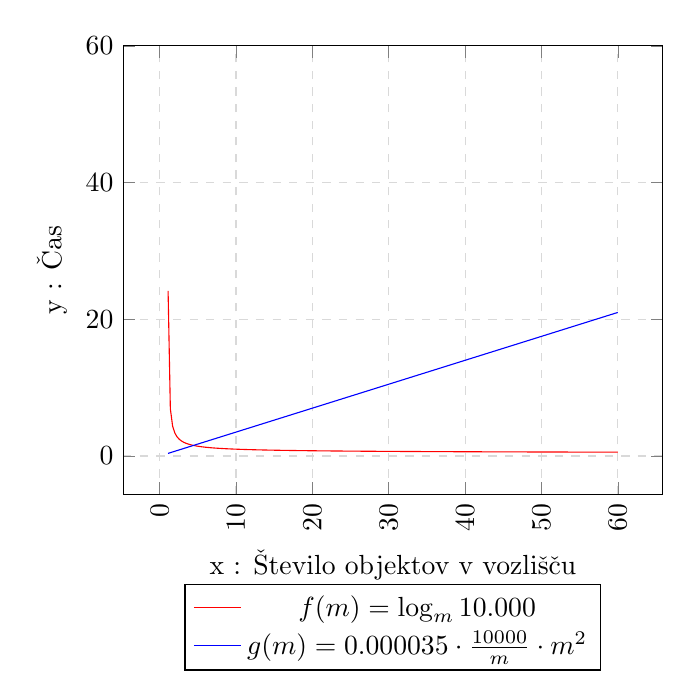
\begin{tikzpicture}
  \begin{axis}[
    %\input{local_pgf_nums.tex}
    domain=1.1:60,
    samples=200,
    grid=major,
    grid style={dashed,gray!30},
    xlabel= x : Število objektov v vozlišču, % Set the labels
    ylabel= y : Čas,
    ymax=60,
    legend style={at={(0.5,-0.2)},anchor=north},
    x tick label style={rotate=90,anchor=east},
    y tick label style={anchor=east, /pgf/number format/fixed},
    cycle list name=color list,
    ]
    % add a plot from table; you select the columns by using the actual name in
    % the .csv file (on top)
    \addplot{(4/log10(x))/4};
    \addplot{0.35 * x};
    \legend{$f(m) =  \log_m{10.000} $, $g(m) = 0.000035 \cdot \frac{10000}{m} \cdot m^2$}
  \end{axis}
\end{tikzpicture}

\end{document}

%table[x=col1,y=col2, col sep=comma] {data/timing_frames.csv}; 